\documentclass[conference,compsoc]{IEEEtran}

\ifCLASSOPTIONcompsoc
  % IEEE Computer Society needs nocompress option
  % requires cite.sty v4.0 or later (November 2003)
  \usepackage[nocompress]{cite}
\else
  % normal IEEE
  \usepackage{cite}
\fi
\ifCLASSINFOpdf
\else
\fi

\usepackage{tikz,pgfplots}
\usepackage{url}

% correct bad hyphenation here
\hyphenation{op-tical net-works semi-conduc-tor}

\begin{filecontents}{lr0.dat}
0.1,1
0.01,2
0.001,2
0.0001,3
0.00001,3
0.000001,4

\end{filecontents}

\begin{filecontents}{lr1.dat}
0.1,1
0.01,2
0.001,2
0.0001,3
0.00001,3
0.000001,4
\end{filecontents}

\begin{filecontents}{lr2.dat}
0.1,1
0.01,2
0.001,2
0.0001,3
0.00001,3
0.000001,4
\end{filecontents}

\begin{filecontents}{lr3.dat}
0.1,1
0.01,2
0.001,2
0.0001,3
0.00001,3
0.000001,4
\end{filecontents}

\begin{filecontents}{l2r0.dat}
0.1,0.458,1,1,1
0.3,0.482,1,1,1
0.5,0.454,1,1,1
\end{filecontents}

\begin{filecontents}{l2r1.dat}
0.1,0.458,1,1,1
0.3,0.482,1,1,1
0.5,0.454,1,1,1
\end{filecontents}

\begin{filecontents}{l2r2.dat}
0.1,0.458,1,1,1
0.3,0.482,1,1,1
0.5,0.454,1,1,1
\end{filecontents}

\begin{filecontents}{l2r3.dat}
0.1,0.458,1,1,1
0.3,0.482,1,1,1
0.5,0.454,1,1,1
\end{filecontents}

\begin{filecontents}{dr0.dat}
8,0.499,1,1,1
8.7,0.505,1,1,1
9.5,0.501,1,1,1
10.3,0.505,1,1,1
\end{filecontents}

\begin{filecontents}{dr1.dat}
8,0.499,1,1,1
8.7,0.505,1,1,1
9.5,0.501,1,1,1
10.3,0.505,1,1,1
\end{filecontents}

\begin{filecontents}{dr2.dat}
8,0.499,1,1,1
8.7,0.505,1,1,1
9.5,0.501,1,1,1
10.3,0.505,1,1,1
\end{filecontents}

\begin{filecontents}{dr3.dat}
8,0.499,1,1,1
8.7,0.505,1,1,1
9.5,0.501,1,1,1
10.3,0.505,1,1,1
\end{filecontents}


\usepackage{pgfplots}

\usepackage{subcaption} 
\usepackage{filecontents}
\begin{document}
%
% paper title
% Titles are generally capitalized except for words such as a, an, and, as,
% at, but, by, for, in, nor, of, on, or, the, to and up, which are usually
% not capitalized unless they are the first or last word of the title.
% Linebreaks \\ can be used within to get better formatting as desired.
% Do not put math or special symbols in the title.
\title{Age Estimation Using Convolutional Neural Networks}


% author names and affiliations
% use a multiple column layout for up to three different
% affiliations
\author{\IEEEauthorblockN{Deniz Rasim Ulug}
\IEEEauthorblockA{School of Computer Engineering\\
Middle East Technical University\\
Ankara, Turkey\\
Email: deniz.ulug@metu.edu.tr}
}





% use for special paper notices
%\IEEEspecialpapernotice{(Invited Paper)}




% make the title area
\maketitle

% As a general rule, do not put math, special symbols or citations

% no keywords




% For peer review papers, you can put extra information on the cover
% page as needed:
% \ifCLASSOPTIONpeerreview
% \begin{center} \bfseries EDICS Category: 3-BBND \end{center}
% \fi
%
% For peerreview papers, this IEEEtran command inserts a page break and
% creates the second title. It will be ignored for other modes.
\IEEEpeerreviewmaketitle



\section{Introduction}
% no \IEEEPARstart
In this report we try to estimate a person's age by the photograph of his face. For this task we use the Machine Learning, and more specifically Convolutional Neural Network(CNN) approach. Our data set consist of 5000 training, and 2000 validation and test images each. We will use a Resnet18 [1] backbone for our architecture and simple Fully Connected (FC) layers on top of it. We will also experiment with Batch Normalization (BN) and Dropout layers.


\section{Architecture}
Our architecture has 2 parts. First, we transform images in to feature vectors of length 512 using Resnet18 with pre-trained weights on ImageNet Dataset [2] . We use the output of the AvgPool layer of Resnet18 for this purpose, which outputs a length 512 vector. 
\\

Then we process these vectors using 1 to 4 number of FC layers, which at the end reduces to a single neuron outputting a single number; the estimation for the age. We also experiment with Dropout and BN layers. The task is a regression task, and we use the standard MSE loss function and RMSprop [3] algorithm for back propagation. 

\section{Choose Of Parameters}

Our model admits variarity of hyper-parameters. Let's examine each of them and briefly explain their duty. For our implementation we used the Pytorch [4] library of Python. 

\subsection{Architecture Parameters}

Our model's architecture admits four important parameters:\\

1) Hidden Layers: The most important "parameter" is the number of hidden layers and the number of neurons per layer. We experimented on the affect of the number of hidden layer with 4 different configuration; 0 to 3 hidden layers. We also tried two different configurations for the number of neurons, "Triangular" and "Rectengular". For Triangualar case we set the number of neurons for each layer in a decreasing order and tried to keep the more or less same ratio of neurons between subsequent layers. Remember that the first layer has 512 neurons and the last layer has 1 neurons. For Rectengular setup, we kept the neuron count per layer as maximum, 512 per se, for each layer. \\

2) Batch Norm Layer: We also tried our model with batch normalization layers, as described in [5]. The BN layer admits on parameters, and we simply drop on BN layer after each FC layer, except for the final layer. The purpose of this is to force each layer to have gaussian activations, therefore BN both increases regularization power and keeps gradients in check. Even tough the BN layer usually used with more traditional activation functions like sigmoid and tanh, we still included this in our experiments in for diversity. \\

3) Dropout Layer: We also experimented with Dropout layers[6], tough only applied them after the input layer and the first hidden layer. A dropout layer randomly zeroes elements of it input tensor, therefore reducing the reliance of the following layer on those elements. In a broader sense, a Dropout layer forces the following layer not to majorly rely on only some small number of prior layer's neurons to make decisions. By this way it increases the generalization power and also again acts as a regularizer.\\

\subsection{Other Parameters}

Aside from the architecture parameters, our model also admits three more important parameters, first two being the optimizer's parameters. \\

1) Learning Rate: This parameter needs no introduction, it is the magnitude of the "step" we take in the direction of gradient at each iteration. \\

2) L2-Regulatization Rate: Likewise a well known one, this is the weight of the L2 regularization in our loss function. \\

3) Batch Size: Batch Size is the number of examples we feed in to our model at each iteration. \\

4) Epoch Count: At each epoch, we feed our model our whole input batch by batch.  Epoch count is the number of times we train our model on our whole training set. We set this to 50, empirically. Higher epoch values cause our model to overfit to training data, giving high accuracy on training set but low accuracy on validation set. Lower values cause our model to underfit, and not converge to local/global minimums. \\

\section{Experiments}

To decide on our final parameters, we did a number of experiments. For each experiment, we varied a single parameter, and set all others to a fixed value, except the number of hidden layers. To make justice to the model, we repeated each experiment for each possible hidden layer count, which are zero to four. After each parameter's experiment, for the subsequent parameters' experiments we used the best value (in terms of accuracy) for that parameter. The default parameters that we start with and their accuracy is given in Table 1.  Note that through this report we run our experiments for 50 epochs and reported the average accuricies of the final 10 epochs. \\

\begin{table}[]
\centering
\caption{Default Parameters}
\label{my-label}
\begin{tabular}{l|ccccccc}
\#Layers & \multicolumn{1}{l}{LR} & \multicolumn{1}{l}{L2} & \multicolumn{1}{l}{\#Neurons} & \multicolumn{1}{l}{Dropout} & \multicolumn{1}{l}{BN} & \multicolumn{1}{l}{BS} & \multicolumn{1}{l}{Acc.} \\ \hline
0 Layer & 0.001 & 0 & {[}{]} & 0 & No & 64 & 0.56 \\ \cline{2-8} 
1 Layer & 0.001 & 0 & {[}128{]} & 0 & No & 64 & 0.59 \\ \cline{2-8} 
2 Layer & 0.001 & 0 & {[}256,64{]} & 0 & No & 64 & 0.59 \\ \cline{2-8} 
3 Layer & 0.001 & 0 & {[}512,128,32{]} & 0 & No & 64 & 0.56
\end{tabular}
\end{table}
1) Learning Rate: \\

The first experiment we did on Learning Rate. All other parameters were set to their default values as showed in Table 1. The results are plotted in figure 1.  We see that for 0-layer and 1-layer architectures the best learning rate was $0.001$ and for 2 and 3 layer architectures it was $0.0001$. So we set learning rate as those values for the subsequent experiments. \\

This difference may be explained such that a higher complexity model, which as a function resides in a higher dimension, may have local minimas which are more saddle like and easier to escape. Also, as was argued in [7], higher complexity model's local minimas has virtually same good performances on test sets. We are merely speculating here.

\begin{figure}
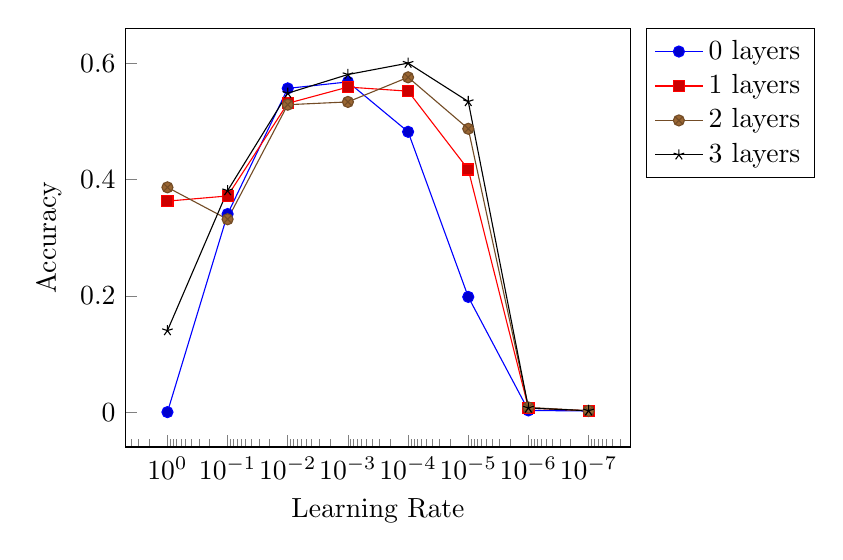
\begin{tikzpicture}
\begin{axis}[xlabel={Learning Rate},ylabel={Accuracy},
legend pos=outer north east,xmode=log, log basis x={10}, xtick pos=left,
ytick pos=left,x dir=reverse,width=8cm]
\addplot coordinates{
(0.0000001,0.002)
(0.000001,0.003)
(0.00001,0.1982)
(0.0001,0.4821)
(0.001,0.5679)
(0.01,0.5568)
(0.1,0.3407)
(1,0.0001)};
\addlegendentry{0 layers}
\addplot coordinates{
(0.0000001,0.0024)
(0.000001,0.0072)
(0.00001,0.4173)
(0.0001,0.552)
(0.001,0.559)
(0.01,0.5311)
(0.1,0.3718)
(1,0.3629)};
\addlegendentry{1 layers}
\addplot coordinates{
(0.0000001,0.0024)
(0.000001,0.0082)
(0.00001,0.4873)
(0.0001,0.5758)
(0.001,0.5335)
(0.01,0.5287)
(0.1,0.3317)
(1,0.3866)};
\addlegendentry{2 layers}
\addplot coordinates{
(0.0000001,0.0024)
(0.000001,0.0072)
(0.00001,0.5342)
(0.0001,0.6002)
(0.001,0.5806)
(0.01,0.5485)
(0.1,0.3809)
(1,0.1403)};
\addlegendentry{3 layers}
\end{axis}
\end{tikzpicture}
\caption{Accuracy versus Learning Rate}
\end{figure}

2) L2-Regularization Rate: As seen in Figure 2, Surprisingly L2 regularization did not have any positive affect  on our accuracy, and for large values decreased our accuracy. For subsequent experiments we did not used the L2 regularization. This result is rather surprising, especially considering that our model will later improve with harsher regularization like dropout. The case may be attributed to the fact that we have relatively low number or neurons in our layers, so sum of their weights may be small regardless. \\

3) Batch Size: Figure 3 shows that as we increase batch size (BS) , our accuracy gets lower and lower. We achieve the best accuracy with the lowest batch size, which is $8$ for us. This is rather saddening since lower batch-sizes are computationally slower. We took the batch size to be $8$ for subsequent experiments. \\ 

Such effect of the BS may be understandable. When we add the gradients to our weights, we in a sense take the average of BS amount of input example. A higher BS means a weaker approximation to a good gradient. Another conjecture argued in [8] says that higher BS values cause our loss function's shape to be "sharper", which leads to poorer generalizations. As the loss function gets sharper, the interval of parameter values of a particular loss-value gets also smaller, so it is easier to miss those intervals. \\

4) Dropout Layer: In figure 4, we applied dropout layers after the input layer and the first hidden layer. Since the number of neurons gets drastically smaller after this, we did not add dropout to subsequent layers. In this figure X axis is the probability of "dropping out" activation of the prior neuron, by equaling them to zero. We see that , similar to L2 regularization, Dropout has very minor positive affects for low probabilities, and negative affects for higher probabilities. Considering conventionally the Dropout layer's probability is taken to be $0.5$, this again shows that our network is quite resilient to over fitting as it is. Since we do not have a hidden layer for the "0-layer" case, Dropout has only negative affect in that case. And for 3-layer case a more complex model means more room for generalization, which a Dropout layer would apply, so 3-layer case shows the best result with $0.3$ dropout probability. For subsequent experiments we apply Dropout with probability $0.2$ to 1 and 2 layer, $0.3$ for 3-layer and $0$ for 0-layer case. \\

5) Batch Norm Layer: In table 2 we show the affect of adding BN layers to our model. This time we add a BN layer to every hidden layer in the model. Since 0-layer configuration has no hidden layers, it is unaffected. Table 2 shows that, for all other configurations Batch Norm had positive affect, so we include BN layers in our subsequent experiments, solely for empirical reasons, but it is also known that BN layers are widely used and helps model to learn correct shifts in means and variances of the activations, which marginally helps the following layer to interpret the activations of the BN layer more rigorously.  \\

\begin{table}[]
\centering
\caption{Batch Norm}
\label{my-label}
\begin{tabular}{l|cc}
\#Layers & \multicolumn{1}{l}{With BN} & \multicolumn{1}{l}{Without BN} \\ \hline
0 Layer  & 0.578                       & 0.578                          \\ \cline{2-3} 
1 Layer  & 0.612                       & 0.611                          \\ \cline{2-3} 
2 Layer  & 0.605                      & 0.609                          \\ \cline{2-3} 
3 Layer  & 0.617                      & 0.622                         
\end{tabular}
\end{table}

6) Number of Neurons:  As mentioned at the prior section, we set the number of neurons per layer in a "Triangular" manner. Now, we would also like to try a more "Rectangular" configuration. The Rectangular configuration has $512$ neuron in each layer. The results are in Table 3. Since increasing the neuron counts makes a more complex model, we reduced the epoch count to 15 and took to average of only the last 5 epochs to report accuracies. Results are drastically worse than Triangular configuration, which are understandable since we have optimizing for Triangular case. \\

One important note is that, in Rectangular configuration accuracies of the training sets (which we have not been reporting) are also drastically higher than the validation set, tough they are not higher than the Triangular case's training set accuracies. This shows that the problem with the Rectangular configuration is an over fit problem, which shows that "regularization trough model" is something that is useful in Triangular case.







\begin{table}[]
\centering
\caption{Triangular versus Rectangular}
\label{my-label}
\begin{tabular}{l|cc}
\#Layers & \multicolumn{1}{l}{Triangular} & \multicolumn{1}{l}{Rectangular} \\ \hline
0 Layer  & 0.578                          & 0.578                           \\ \cline{2-3} 
1 Layer  & 0.611                          & 0.542                           \\ \cline{2-3} 
2 Layer  & 0.609                          & 0.464                           \\ \cline{2-3} 
3 Layer  & 0.622                          & 0.5355                         
\end{tabular}
\end{table}

\begin{figure}
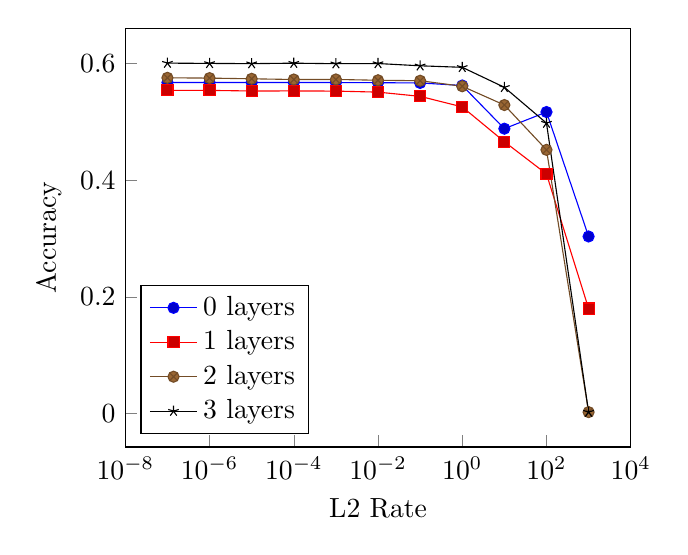
\begin{tikzpicture}
\begin{axis}[xlabel={L2 Rate},ylabel={Accuracy},
legend pos=south west,xmode=log, log basis x={10}, xtick pos=left,
ytick pos=left,width=8cm]
\addplot coordinates{
(1000,0.3037)
(100,0.5172)
(10,0.4886)
(1,0.5627)
(0.1,0.5671)
(0.01,0.5675)
(0.001,0.5678)
(0.0001,0.5679)
(0.00001,0.5679)
(0.000001,0.5679)
(0.0000001,0.5679)
};
\addlegendentry{0 layers}
\addplot coordinates{
(1000,0.18)
(100,0.4110)
(10,0.4663)
(1,0.5260)
(0.1,0.5441)
(0.01,0.55135)
(0.001,0.5531)
(0.0001,0.5534)
(0.00001,0.5533)
(0.000001,0.5543)
(0.0000001,0.5544)
};
\addlegendentry{1 layers}
\addplot coordinates{
(1000,0.0024)
(100,0.4523)
(10,0.5292)
(1,0.5614)
(0.1,0.5709)
(0.01,0.5717)
(0.001,0.5731)
(0.0001,0.5730)
(0.00001,0.5742)
(0.000001,0.5754)
(0.0000001,0.5759)
};
\addlegendentry{2 layers}
\addplot coordinates{
(1000,0.0024)
(100,0.4982)
(10,0.5596)
(1,0.5939)
(0.1,0.5965)
(0.01,0.6004)
(0.001,0.6001)
(0.0001,0.6010)
(0.00001,0.6002)
(0.000001,0.6006)
(0.0000001,0.6011)
};
\addlegendentry{3 layers}
\end{axis}
\end{tikzpicture}
\caption{Accuracy versus L2 Rate}
\end{figure}


\begin{figure}
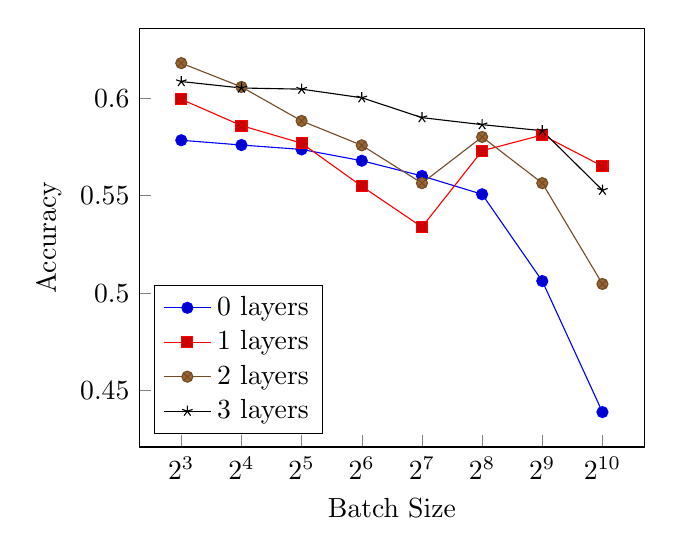
\begin{tikzpicture}
\begin{axis}[xlabel={Batch Size},ylabel={Accuracy},
legend pos=south west, xtick pos=left,
ytick pos=left,width=8cm,
xmode=log, log basis x={2},
xtick={8,16,32,64,128,256,512,1024}
]
\addplot coordinates{
(8,0.5784)
(16,0.57595)
(32,0.5737)
(64,0.5679)
(128,0.5601)
(256,0.5507)
(512,0.5062)
(1024,0.4390)
};
\addlegendentry{0 layers}
\addplot coordinates{
(8,0.5994)
(16,0.5859)
(32,0.5769)
(64,0.5548)
(128,0.5339)
(256,0.5730)
(512,0.5811)
(1024,0.5651)
};
\addlegendentry{1 layers}
\addplot coordinates{
(8,0.61795)
(16,0.60575)
(32,0.5883)
(64,0.5758)
(128,0.5564)
(256,0.5801)
(512,0.5564)
(1024,0.5047)
};
\addlegendentry{2 layers}
\addplot coordinates{
(8,0.6085)
(16,0.6052)
(32,0.6046)
(64,0.6002)
(128,0.5900)
(256,0.5864)
(512,0.5833)
(1024,0.5528)
};
\addlegendentry{3 layers}
\end{axis}
\end{tikzpicture}
\caption{Accuracy versus Batch Size}
\end{figure}

\begin{figure}
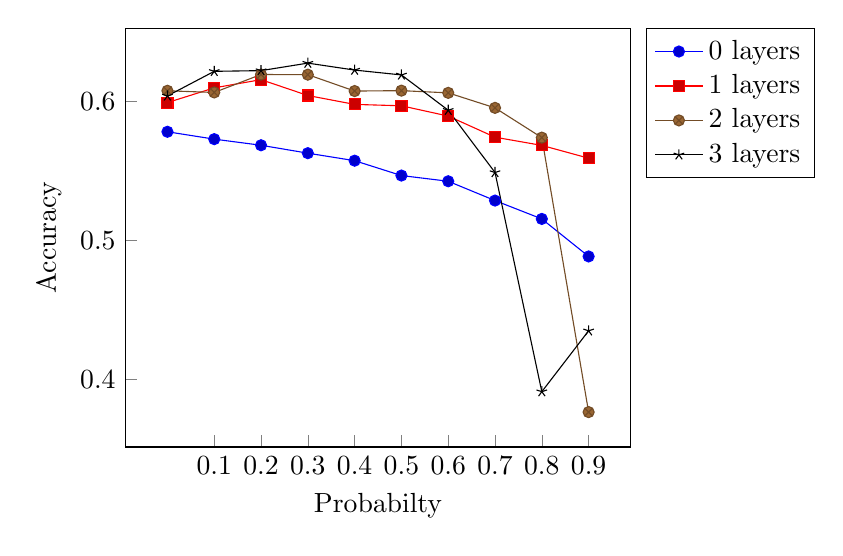
\begin{tikzpicture}
\begin{axis}[xlabel={Probabilty},ylabel={Accuracy},
legend pos=outer north east, xtick pos=left,
ytick pos=left,width=8cm,
xtick={0.1,0.2,0.3,0.4,0.5,0.6,0.7,0.8,0.9}
]
\addplot coordinates{
(0,0.5784)
(0.1,0.5731)
(0.2,0.5687)
(0.3,0.563)
(0.4,0.5576)
(0.5,0.5469)
(0.6,0.5428)
(0.7,0.5289)
(0.8,0.5157)
(0.9,0.4887)
};
\addlegendentry{0 layers}
\addplot coordinates{
(0,0.5994)
(0.1,0.6100)
(0.2,0.6159)
(0.3,0.6045)
(0.4,0.5981)
(0.5,0.5971)
(0.6,0.5897)
(0.7,0.5745)
(0.8,0.5686)
(0.9,0.5594)

};
\addlegendentry{1 layers}
\addplot coordinates{
(0,0.6079)
(0.1,0.6067)
(0.2,0.6196)
(0.3,0.6195)
(0.4,0.6077)
(0.5,0.6080)
(0.6,0.6064)
(0.7,0.5956)
(0.8,0.5742)
(0.9,0.3767)
};
\addlegendentry{2 layers}
\addplot coordinates{
(0,0.6042)
(0.1,0.6219)
(0.2,0.6224)
(0.3,0.6278)
(0.4,0.6228)
(0.5,0.6193)
(0.6,0.5939)
(0.7,0.5491)
(0.8,0.3914)
(0.9,0.4352)
};
\addlegendentry{3 layers}
\end{axis}
\end{tikzpicture}
\caption{Accuracy versus Dropout Probabilty}
\end{figure}


\section{Best Model}

Now that we have determined the best parameters empirically, we give our final parameters and their accuracies in Table 4.

\begin{table}[]
\centering
\caption{Best Parameters}
\label{my-label}
\begin{tabular}{l|ccccccc}
\#Layers & \multicolumn{1}{l}{LR} & \multicolumn{1}{l}{L2} & \multicolumn{1}{l}{\#Neurons} & \multicolumn{1}{l}{Dropout} & \multicolumn{1}{l}{BN} & \multicolumn{1}{l}{BS} & \multicolumn{1}{l}{Acc.} \\ \hline
0 Layer & 0.001 & 0 & {[}{]} & 0 & - & 8 & 0.578 \\ \cline{2-8} 
1 Layer & 0.001 & 0 & {[}128{]} & 0.2 & No & 8 & 0.611 \\ \cline{2-8} 
2 Layer & 0.0001 & 0 & {[}256,64{]} & 0.2 & No & 8 & 0.609 \\ \cline{2-8} 
3 Layer & 0.0001 & 0 & {[}512,128,32{]} & 0.3 & No & 8 & 0.622
\end{tabular}
\end{table}

Also Figure 5 shows the loss graphics, and figure 6 shows the accuracy graphics for 100 epochs. We chose 3-layer configuration as our final model, as it gave the best results consistently. As expected, after around 40 epochs model starts to over fit, the difference between validation and training loss and accuracy gets bigger and bigger. This is the expected behavior. \\

We also see our loss and accuracy decrease and increase, respectively, smoothly, which means our model successfully learns and smoothly converges to whatever local minima it finds.

\begin{figure}
  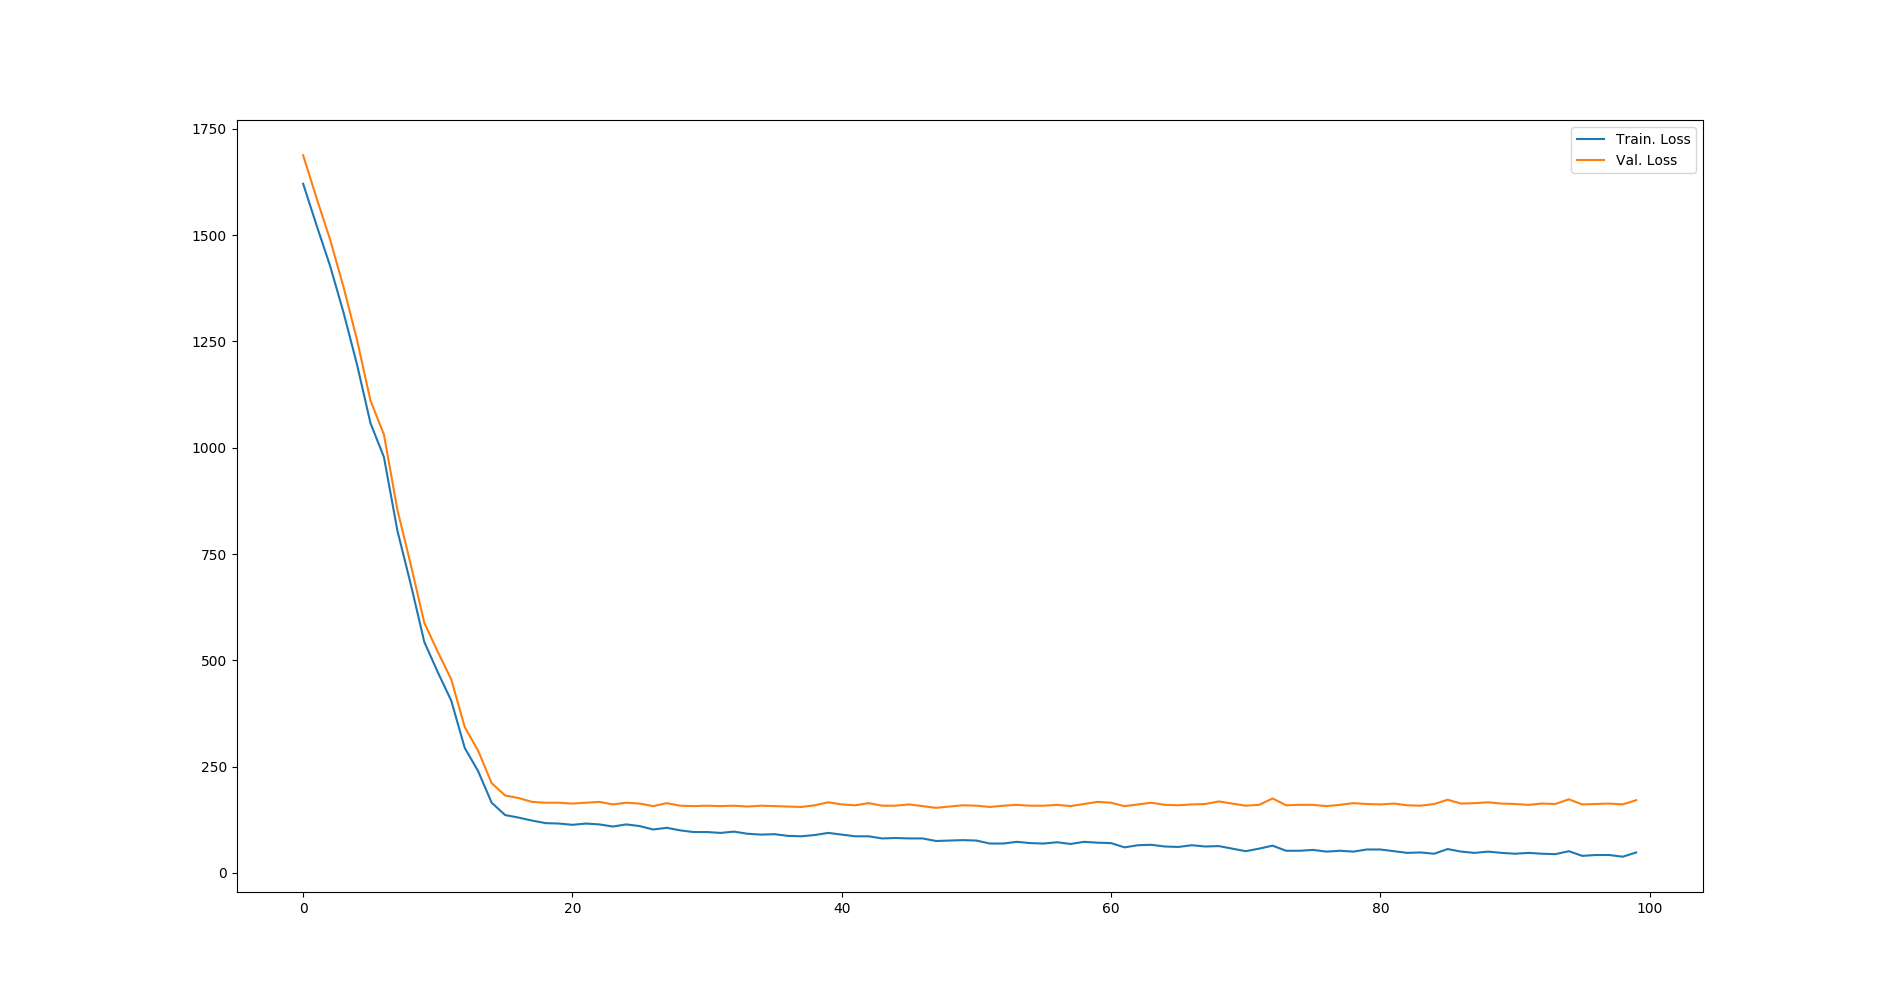
\includegraphics[width=\linewidth]{loss.png}
  \caption{Loss Graphic}
  \label{fig:boat1}
\end{figure}

\begin{figure}
  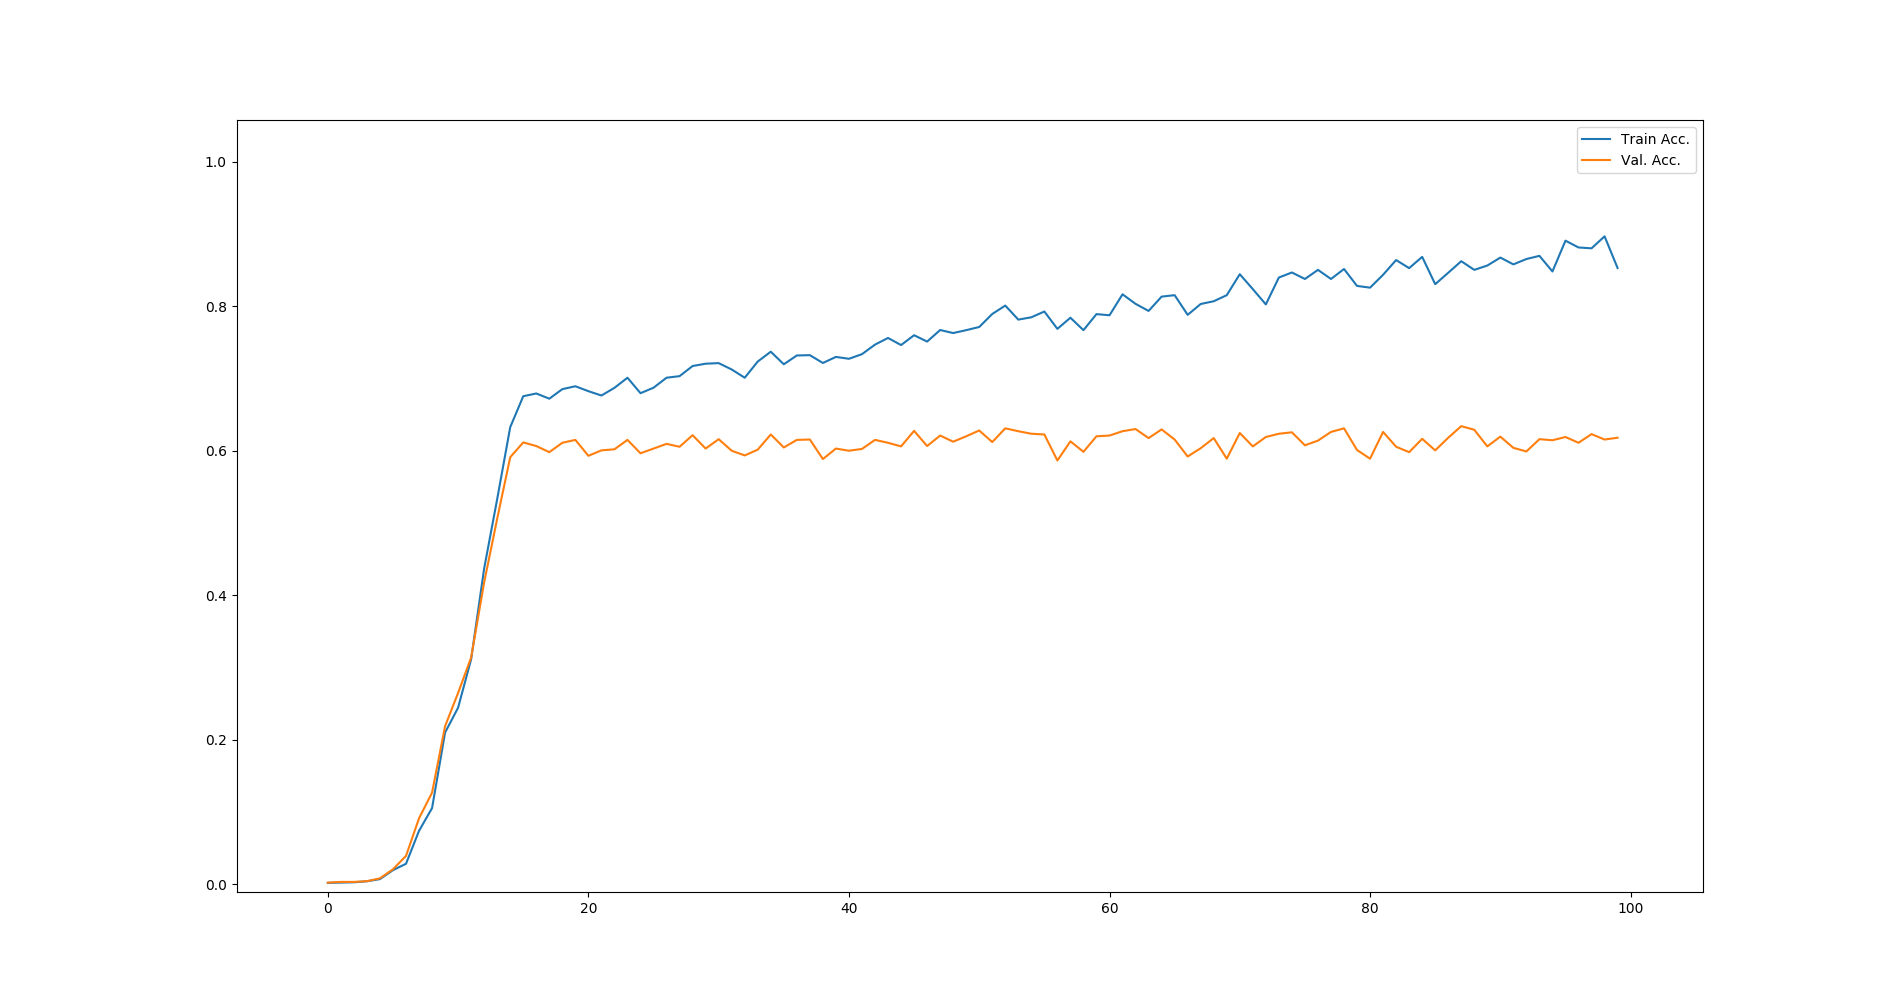
\includegraphics[width=\linewidth]{acc.png}
  \caption{Accuracy Graphic}
  \label{fig:boat1}
\end{figure}

\section{Qualitative Assessment}

Figure 10 shows the qualitative pictures, predictions are given in captions. We used glass and hat to emulate occlusion, and tried two different pose for each set; straight looking and left looking. \\

As seen in figure , our models consistently predicts the same age range for all occlusion and poses. Even tough the person's age is 22, he admittedly looks in his 30s, specially considering the beard. So we take the prediction to be quite successful given the person indeed looks in his 30s, but maybe lower predictions would have been better. We take this to be in expected error range. \\

It is nice that the predictions are consistent and similar even with those wild accessories. \\

\begin{figure}[h!]
  \centering
  \begin{subfigure}[b]{0.4\linewidth}
    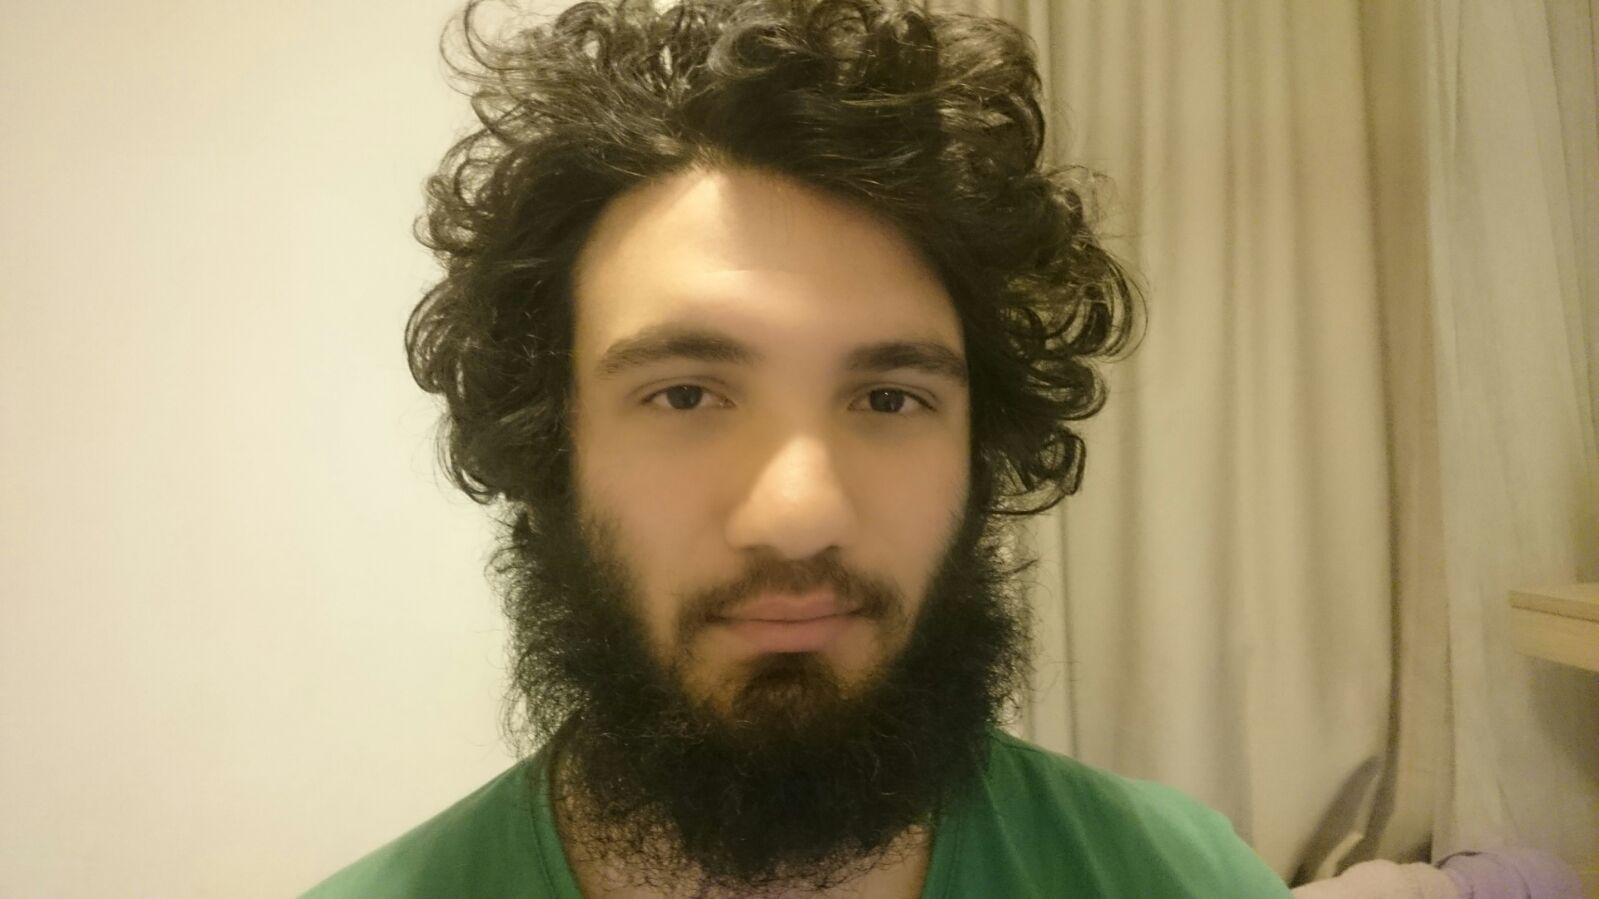
\includegraphics[width=\linewidth]{11.jpeg}
    \caption{37}
  \end{subfigure}
  \begin{subfigure}[b]{0.4\linewidth}
    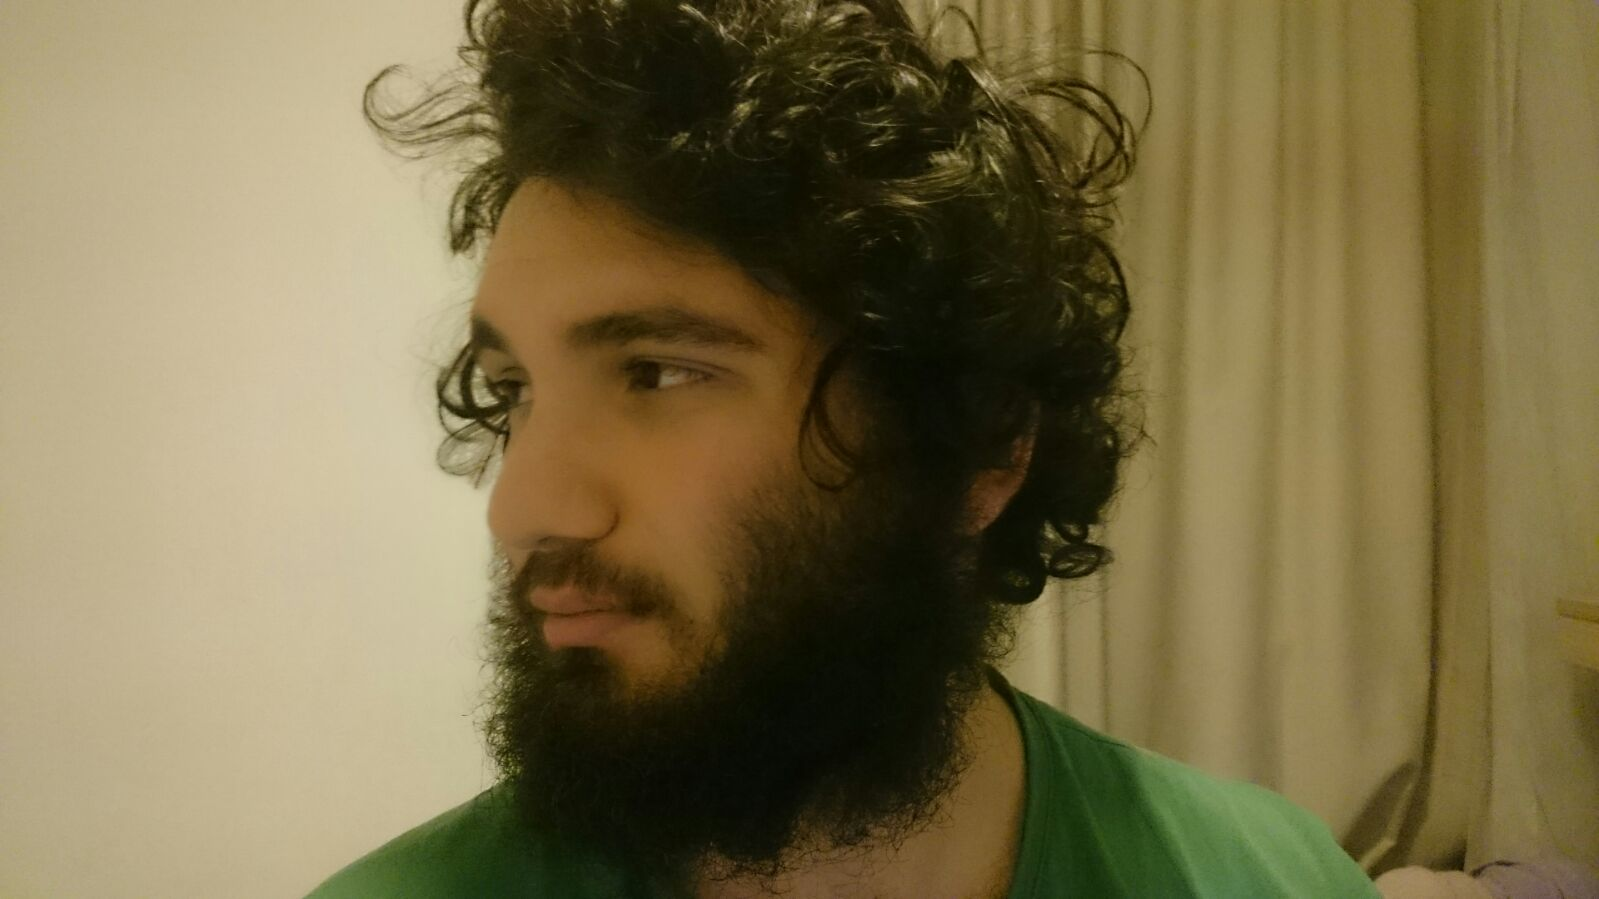
\includegraphics[width=\linewidth]{22.jpeg}
    \caption{36}
  \end{subfigure}


\end{figure}

\begin{figure}[h!]
  \centering
  \begin{subfigure}[b]{0.4\linewidth}
    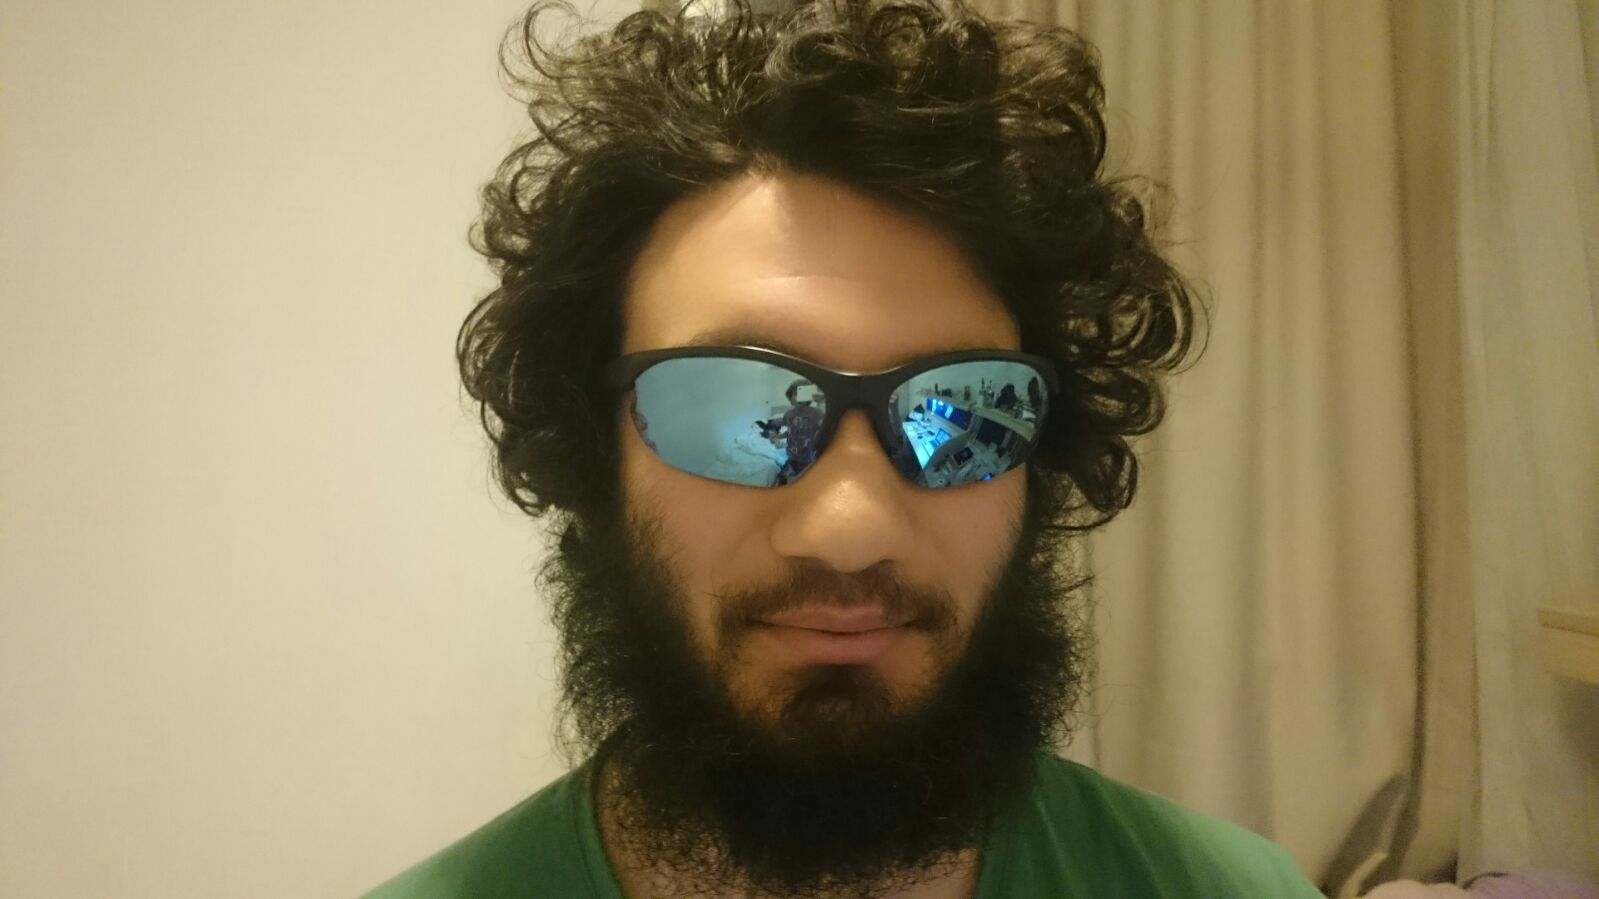
\includegraphics[width=\linewidth]{33.jpeg}
    \caption{38}
  \end{subfigure}
  \begin{subfigure}[b]{0.4\linewidth}
    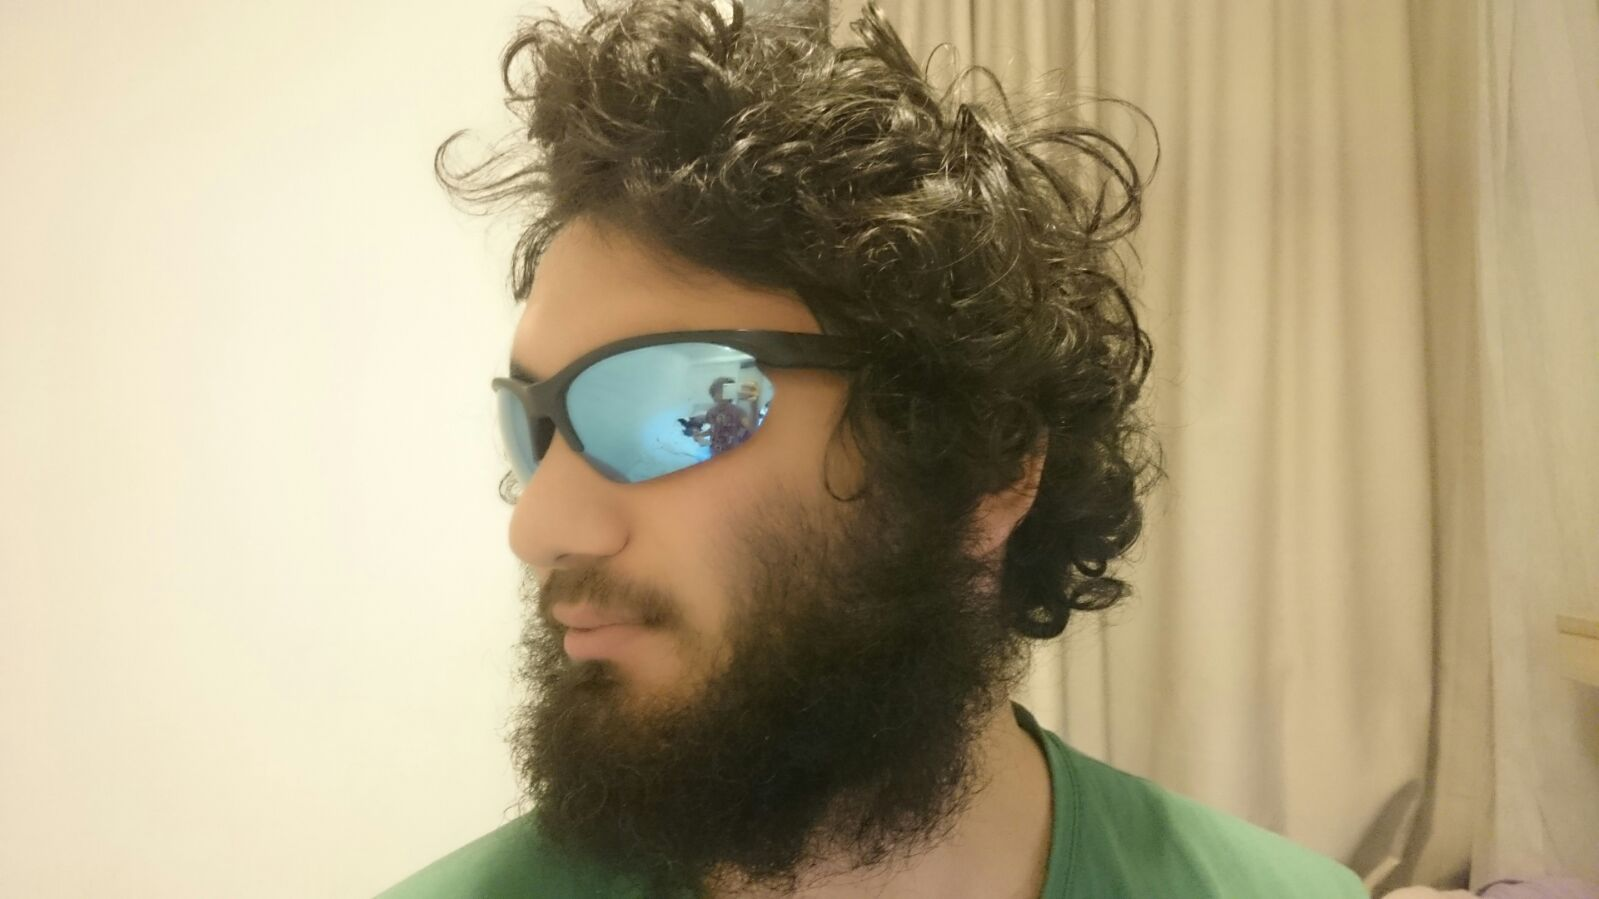
\includegraphics[width=\linewidth]{44.jpeg}
    \caption{34}
  \end{subfigure}

\end{figure}

\begin{figure}[h!]
  \centering
  \begin{subfigure}[b]{0.4\linewidth}
    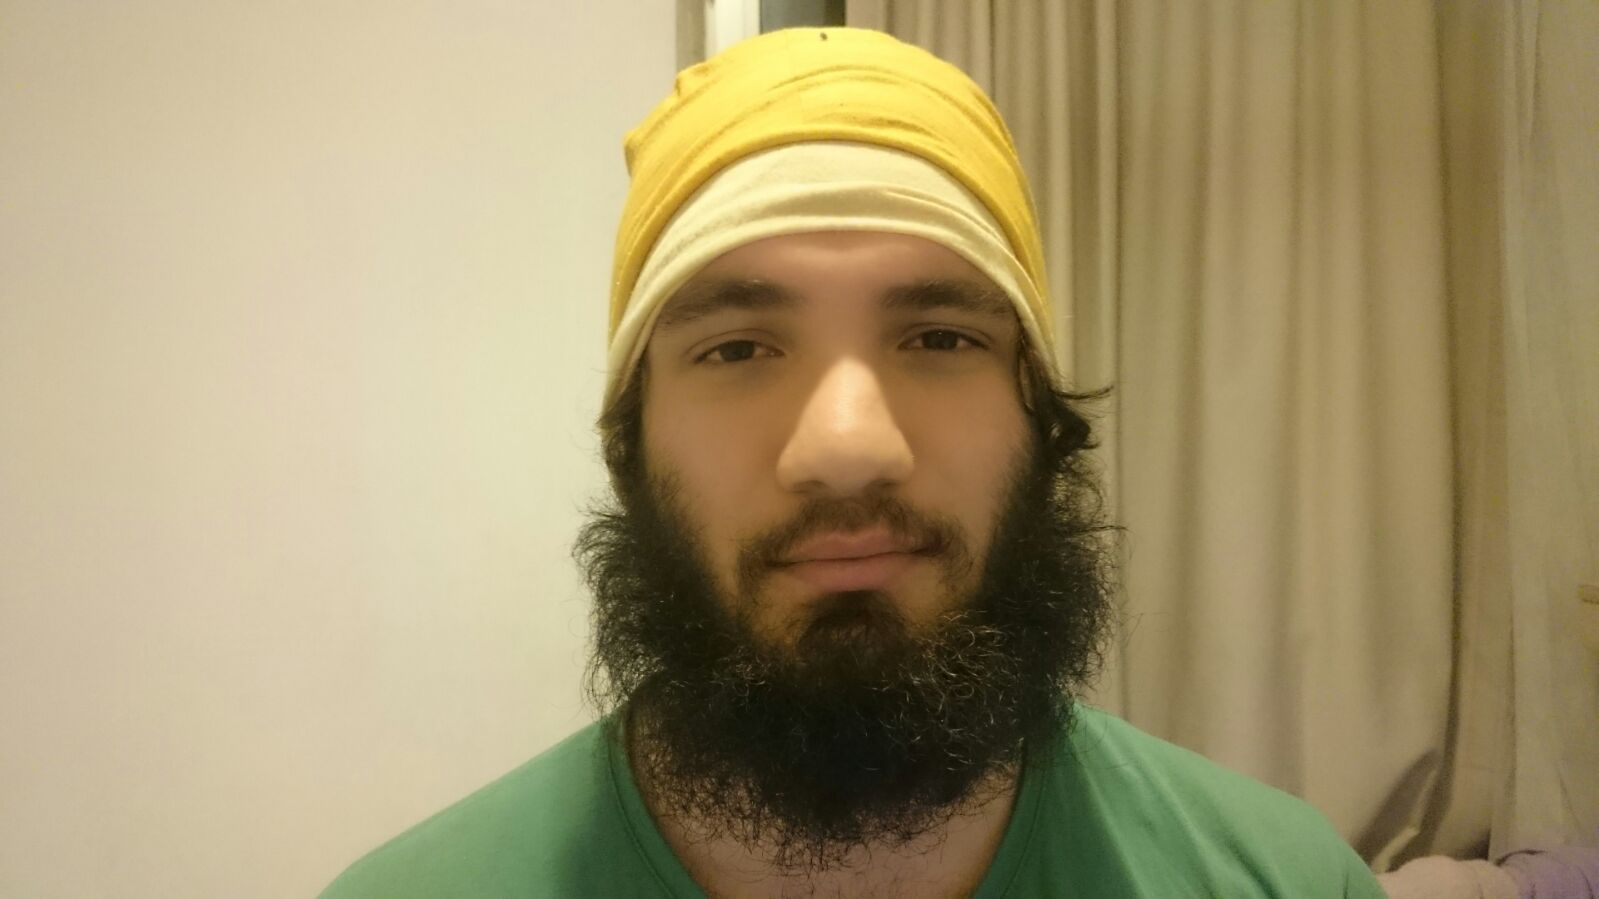
\includegraphics[width=\linewidth]{55.jpeg}
    \caption{33}
  \end{subfigure}
  \begin{subfigure}[b]{0.4\linewidth}
    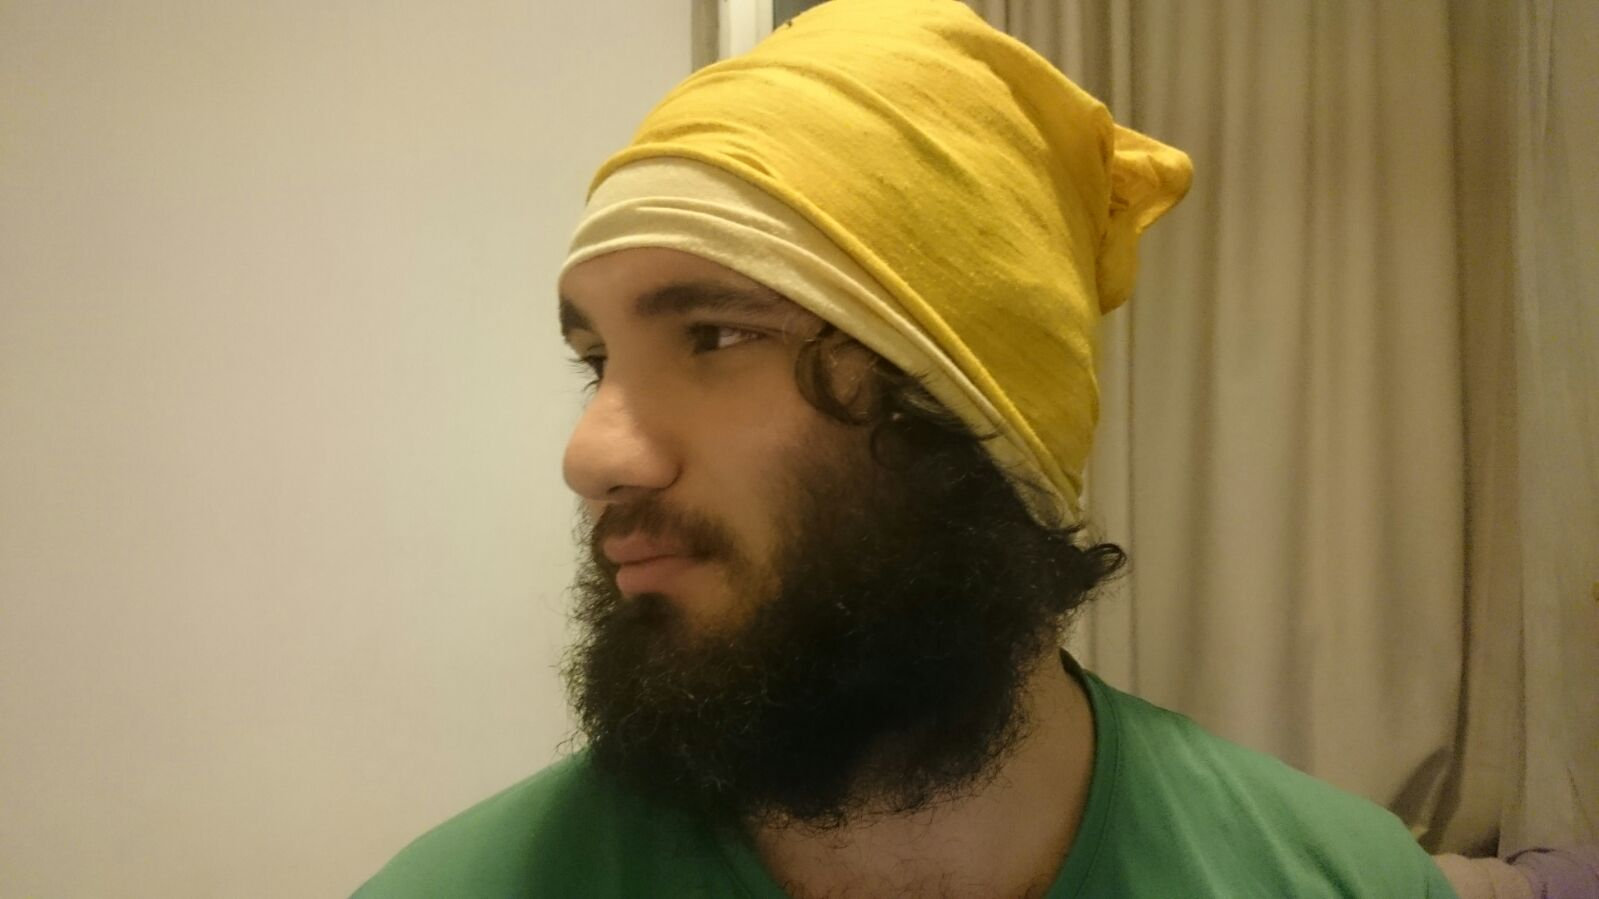
\includegraphics[width=\linewidth]{66.jpeg}
    \caption{36}
  \end{subfigure}

\end{figure}

\begin{figure}[h!]
  \centering
  \begin{subfigure}[b]{0.4\linewidth}
    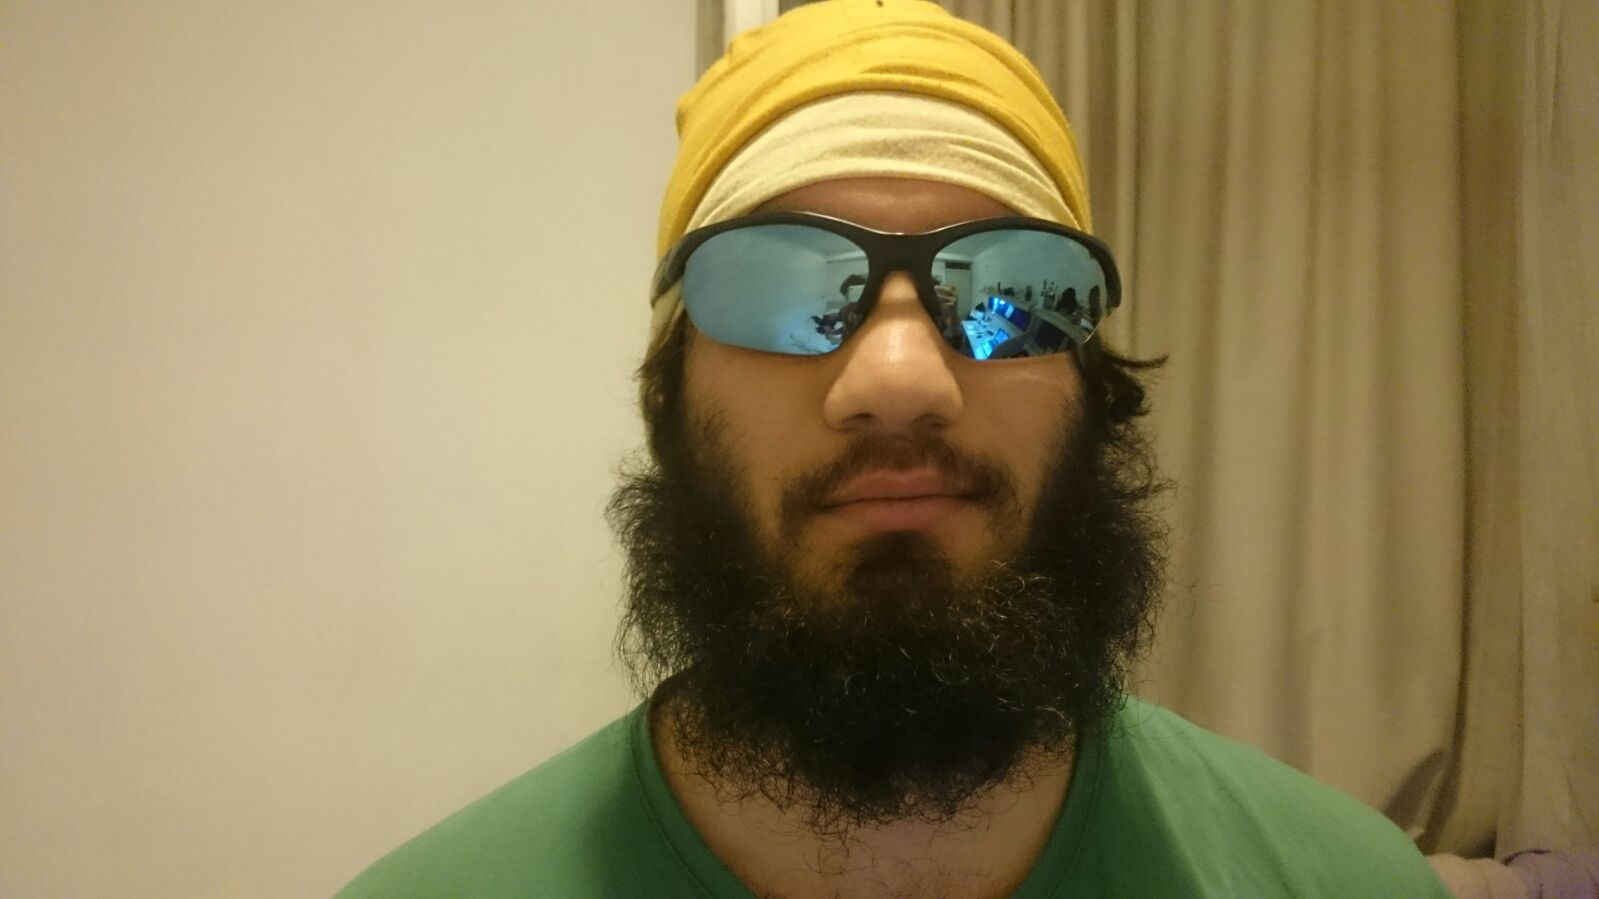
\includegraphics[width=\linewidth]{77.jpeg}
    \caption{33}
  \end{subfigure}
  \begin{subfigure}[b]{0.4\linewidth}
    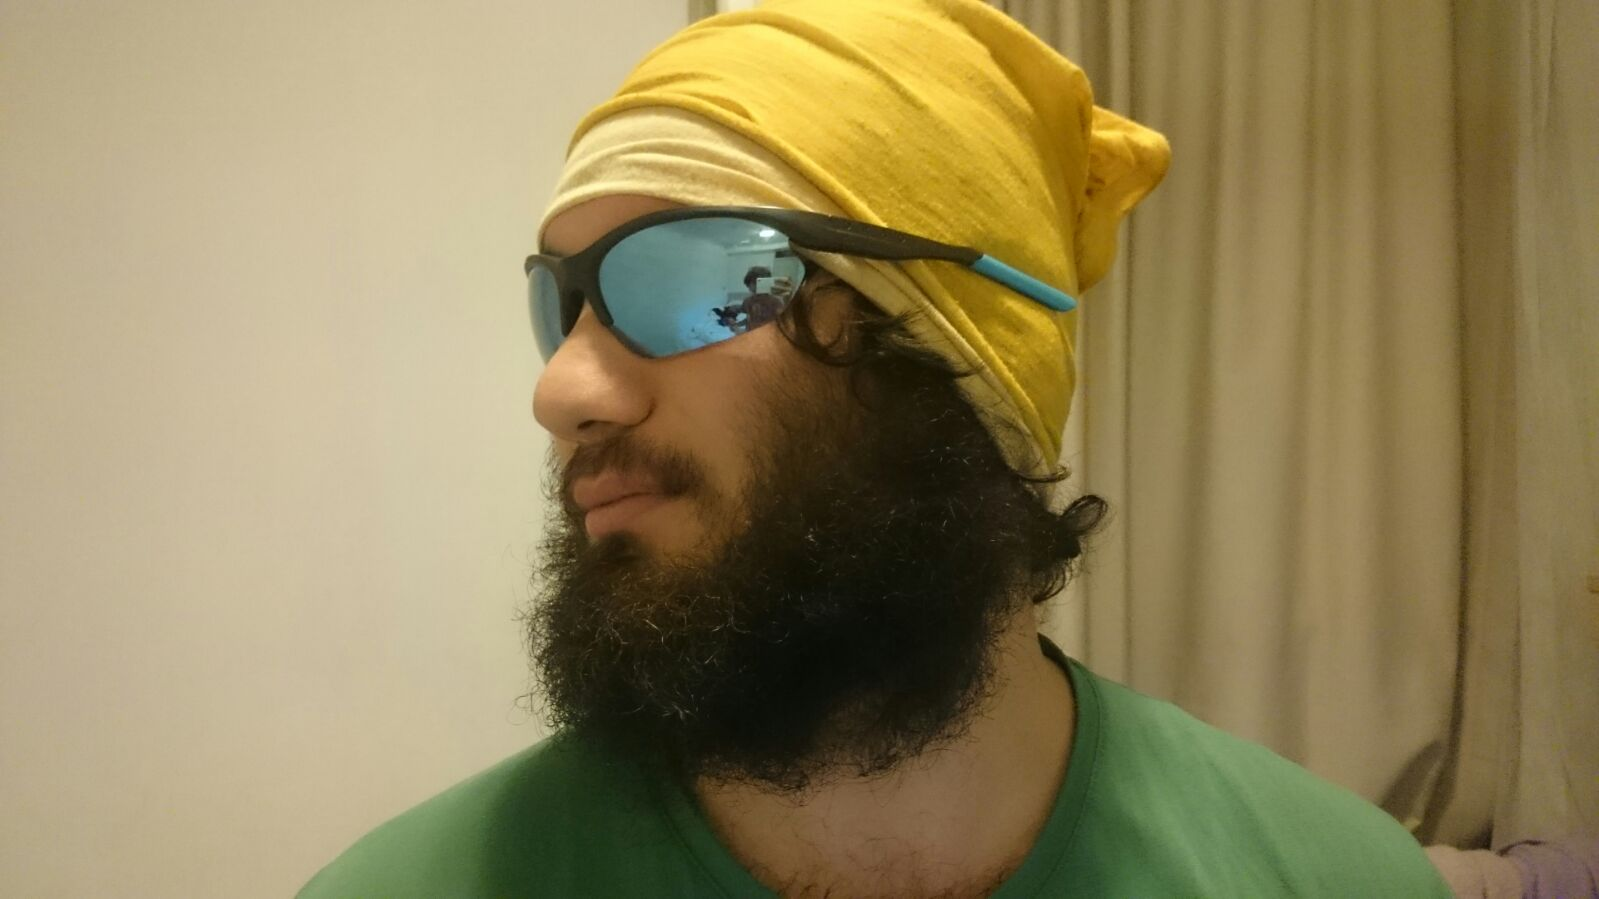
\includegraphics[width=\linewidth]{88.jpeg}
    \caption{35}
  \end{subfigure}
  \caption{Qualitative Assesment with pictures with different occlusions/poses }

\end{figure}

\section{Future Work}
We may add that our research can be immediately extended in the following ways; \\

1) We tried a rectangular configuration but did not search its parameter space properly, also we did not properly experimented with different neuron counts. This may be investigated to come up with better base-models. \\

2) We approached the problem as a regression task, but since we evalute our succes with a margin of error of 5, and since the age of people are limited, the same task can be tried as a classification task.

\section{Conclusion}

In this work, we tried to approach the age estimation problem with CNN coupled with differen fully connected heads. Result accuracies are good, and the assesment pictures shows consistency through occlusion and pose. We experimented with many different parameter settings, and achieved a mean accuracy of $\%60$ with our best parameters.

\begin{thebibliography}{1}


\bibitem{IEEEhowto:kopka} 
	He, K., Zhang, X., Ren, S., \& Sun, J. (2016). Deep residual learning for image recognition. In Proceedings of the IEEE conference on computer vision and pattern recognition (pp. 770-778).
\bibitem{IEEEhowto:kopka} 
	Russakovsky, O., Deng, J., Su, H., Krause, J., Satheesh, S., Ma, S., ... \& Berg, A. C. (2015). Imagenet large scale visual recognition challenge. International Journal of Computer Vision, 115(3), 211-252.
\bibitem{IEEEhowto:kopka} 
	Hinton, G., Srivastava, N., \& Swersky, K. (n.d.). Neural Networks for Machine Learning. Retrieved from \url{www.cs.toronto.edu/~tijmen/csc321/slides/lecture_slides_lec6.pdf}
Originally introduced in his lectures and does not have its own paper.
\bibitem{IEEEhowto:kopka} 
	Paszke, A., Gross, S., Chintala, S., Chanan, G., Yang, E., DeVito, Z., ... \& Lerer, A. (2017). Automatic differentiation in PyTorch.
\bibitem{IEEEhowto:kopka} 
	Ioffe, S., \& Szegedy, C. (2015). Batch normalization: Accelerating deep network training by reducing internal covariate shift. arXiv preprint arXiv:1502.03167.
\bibitem{IEEEhowto:kopka} 
	Srivastava, N., Hinton, G., Krizhevsky, A., Sutskever, I., \& Salakhutdinov, R. (2014). Dropout: A simple way to prevent neural networks from overfitting. The Journal of Machine Learning Research, 15(1), 1929-1958.
\bibitem{IEEEhowto:kopka} 	
	Choromanska, A., Henaff, M., Mathieu, M., Arous, G. B., \& LeCun, Y. (2015, February). The loss surfaces of multilayer networks. In Artificial Intelligence and Statistics (pp. 192-204).
\bibitem{IEEEhowto:kopka} 		
	Keskar, N. S., Mudigere, D., Nocedal, J., Smelyanskiy, M., \& Tang, P. T. P. (2016). On large-batch training for deep learning: Generalization gap and sharp minima. arXiv preprint arXiv:1609.04836.
\end{thebibliography}

\end{document}


